% LaTeX Template for Project Report, Version 2.0
% (Abstracted from a Major Project Report at CSED, NIT Calicut but can be
% modified easily to use for other reports also.)
%
% Released under Creative Commons Attribution license (CC-BY)
% Info: http://creativecommons.org/licenses/by/3.0/
%
% Created by: Kartik Singhal
% BTech CSE Batch of 2009-13
% NIT Calicut
% Contact Info: kartiksinghal@gmail.com
%
% It is advisable to learn the basics of LaTeX before using this template.
% A good resource to start with is http://en.wikibooks.org/wiki/LaTeX/
%
% All template fields are marked with a pair of angular brackets e.g. <title here>
% except for the ones defining citation names in ref.tex.
%
% Empty space after chapter/section/subsection titles can be used to insert text.
%
% Just compile this file using pdflatex after making all required changes.

\documentclass[12pt,a4paper]{report}
\renewcommand{\baselinestretch}{1.5} 
\usepackage[titletoc]{appendix}
\usepackage{float}
\usepackage{listings}
\usepackage{setspace}
\usepackage{longtable}
\usepackage{color}
\usepackage{ragged2e}
\usepackage{listings}
\usepackage{amsmath}
\usepackage{caption}
\usepackage[pdftex]{graphicx} %for embedding images
\usepackage{url} %for proper url entries
\usepackage[bookmarks, colorlinks=false, pdfborder={0 0 0}, pdftitle={ASAGS_report}, pdfauthor={sekhar}, pdfsubject={<subject here>}, pdfkeywords={<keywords here>}]{hyperref} %for creating links in the pdf version and other additional pdf attributes, no effect on the printed document
%\usepackage[final]{pdfpages} %for embedding another pdf, remove if not required

\begin{document}
\renewcommand\bibname{References} %Renames "Bibliography" to "References" on ref page

%include other pages
\pagenumbering{roman} %numbering before main content starts
\cleardoublepage
%\pagebreak
\phantomsection
\addcontentsline{toc}{chapter}{Certificate}
\chapter*{Certificate}
\vspace{1.0in}

\newpage

\cleardoublepage
%\pagebreak
\phantomsection
\addcontentsline{toc}{chapter}{Declaration}
\chapter*{Declaration}
\vspace{1.0in}

\newpage

\cleardoublepage
%\pagebreak
\phantomsection
\addcontentsline{toc}{chapter}{Acknowledgements}
\chapter*{Acknowledgments}
\vspace{-0.55in}
We would like to express our deep-felt appreciation and gratitude to \textbf{Mrs. E Padmalatha}, our project guide, for his skilful guidance, constant supervision, timely suggestion, keen interest and encouragement in completing the individual seminar within the stipulated time.
\par
We wish to express our gratitude to \textbf{Dr. T Sridevi} and \textbf{Mr. J Shiva Sai}, Project Coordinators, who have shown keen interest and even rendered their valuable time and guidance in terms of suggestions and encouragement
\par
We are honored to express our profound sense of gratitude to \textbf{Dr. M Swamy Das}, Head of Department, CSE, who has served as a host of valuable corrections and for providing us time and amenities to complete this project.
\par
We gratefully express our thanks to \textbf{Dr. P Ravinder Reddy}, Principal of our college and the management of CHAITANYA BHARATHI INSTITUTE OF TECHNOLOGY for providing excellent academic and learning environment in the college.
\par
We wish to express our heartfelt gratitude to the Members of Staff and all others who helped us in bringing up our project. We would also like to thank the Lab assistants and Programmers for helping us through our project.
\\
\begin{flushright}
\textbf{Karedla Anantha Sashi Sekhar}\\\textbf{160114733091}\\\textbf{Dasarada Ram Reddy Mudiam}\\\textbf{160114733092}
\end{flushright}
\newpage

\vspace{2in}
\begin{abstract}

A large number of people gathered together and arranged in an unruly manner is known as a crowd. Monitoring the events taking place in the presence of crowd is of utmost importance. Today it is done manually by a human surveyor with the help of CCTV cameras. Our idea is to reduce the burden on the human surveyor by automating the process of detecting disturbance in the crowd. Critical amount of time may be saved by detecting disturbance in crowd instantaneously. This critical time we save may be the difference between life and death. This disturbance may be caused by any event such as bomb blast, fire, riots etc. This project focuses on implementation of an algorithm that can detect disturbance in the crowd. It considers flow-vector magnitudes change over time for a short set of frames to statistically determine whether those short set of frames are violent or non-violent. The challenge in this project is to keep the processing quick and real time, an alert should be generated within few seconds of change in crowd behaviour. 


\end{abstract} 


\tableofcontents
\listoffigures
\listoftables

\newpage
\pagenumbering{arabic} %reset numbering to normal for the main content

\chapter{Problem Definition}

Automation in Real-Time Analysis of crowd can make surveillance more efficient. In this modern era, the number of cameras for surveillance is continuously increasing which leads to increase in burden on the human. Real time alert generation is a system that can analyse abnormalities accurately in real time and create an alert. These automatic alerts may help to react quickly and cause less damage to civilians and the property.

\chapter{Introduction}

\section{Problem Statement}
Automation in Real-Time analysis of crowd can make surveillance more efficient. In this modern era, the number of cameras for surveillance is continuously increasing which leads to increase in burden on the human. Real Time alert generation is a system that can analyse abnormalities accurately in real time and create an alert. These automatic alerts may help to proact rather than to react. 

\section{Objective}
Public safety is an important concern for any organization. So as to achieve that an organization takes the help of CCTV cameras. With the decrease in price of cameras, amount of information generated in terms of cctv footage is huge. Real time processing of this footage is required so that the burden on the human surveyors may be decreased.
\par
Aim of this project is to implement an algorithm that can process the incoming footage in real time and detect disturbance within few seconds of an abnormal activity. Crucial amount of time will be saved if an alert is generated. This time may be the difference between the life and death of a person.

\section{Motivation}
Crowd can be defined as a large number of people in close proximity to each other. Whenever an abnormal event happens occurs in crowd, all the people in present the crowd react to that at once. This gives us opportunity to  detect violence in crowd if we detect that exact moment where the abnormal activity happens.
\par 
If an alert is generated during the exact moment when the outburst takes place, it may be used to alert the local bodies such as riot control team to take control of the situation. It would be highly beneficial for us to detect violence at the moment of detection rather than reacting to the incident later on.

\section{Existing System}
Now-a-days every public area will have CCTV coverage so as to protect the public. In the existing manual surveillance system, a human surveyor continuously pays attention to screens, as the number of cameras increase burden on the human will also increase. This system is laggy and it may or may not detect every  outbreak. 
\par
Violence detection is a part of “Action Recognition”. There has been intensive research on action recognition in the past. Much research has been done in person to person fight detection, sports violence detection, violence detection in movies and slow motion fight detection. Violence detection in crowd is one of the most trending topics in the area of action recognition. 
\par
Existing Person-to-Person fight detection takes heavy computational power and cannot be refined to be used in real-time detection. Blob method used is quick and requires less computational power but it can be used for only Person-to-Person fight detection, we cannot refine it to be used for crowd violence detection.
\subsection{Problems in Existing System}
\begin{itemize}
	\item As the number of cameras increase burden on the human will also increase. This system is laggy and it may or may not detect every  outbreak.
	\item Existing Person-to-Person fight detection takes heavy computational power and cannot be refined to be used in real-time detection.
	\item Blob method used is quick and requires less computational power but it can be used for only Person-to-Person fight detection, we cannot refine it to be used for crowd violence detection.
\end{itemize}
\section{Proposed System}
\begin{itemize}
  \item We propose an automated system to detect and generate alert in real time incase outbreak of violence in crowd using Video Processing, Optical Flow and Violent Flow Descriptors(ViF). 
  \item In the proposed system, surveillance videos are taken as input and output is detection of violence(if present) in the video.
  \item Our system works in real time i.e it detects disturbance or violence in crowd present in the video within milliseconds of outset of violence. 
  \item The Real time detection of violence helps to proact rather than to react.
\end{itemize}
\section{Organisation of Project Report}
This project report is mainly divided into 6 modules as follows:
\begin{itemize}
  \item The second chapter deals with the Introduction of the Project and explanation about some basic concepts.
  \item The third chapter discusses about the literature survey of this project which includes an insight into the core concepts of our project.
  \item Fourth chapter deals with the Hardware and Software requirements of the project.
  \item Fifth chapter gives the methodology of the project, the way proposed algorithm is generated.
  \item Sixth chapter gives details of the "in the wild" dataset.
  \item The seventh chapter deals with the design of our proposed system. 
  \item The eighth chapter deals with the implementation of our system which discusses about the algorithms used in building our system.
  \item The ninth chapter displays our results and discussions through a series of screenshots. 
  \item From tenth chapter onwards details about the conclusions, future scope of our project and the limitations. 
\end{itemize}


 
\chapter{Literature Survey}
% \begin{table}
% \begin{center}
% \begin{tabular}{|p{3cm}|p{3cm}|p{2cm}|p{4cm}|p{3cm}|}
% \hline
% \textbf{Title} & \textbf{Methodology} & \textbf{Results} & \textbf{Merits}  & \textbf{Demerits}\\
% \hline
% Violence detection using Oriented Violent Flows, 2016 [1] & AdaBoost and SVM classifier. & 88.00 percent & Feature representation model, which depicts the information involving both the motion magnitude and motion orientation. & Detection point where the behaviour is changing from normal to abnormal is time consuming.\\
% \hline
% Violent Flows:Real-Time Detection of Violent Crowd Behaviour, 2012 [2] & Global descriptors and SVM classifier & 5-fold cross validation: 81.30 percent & The algorithm detected far more violent scenes correctly, compared to existing work. It was furthermore far faster to detect the violence, typically in less than a second from its outbreak & Only magnitude of the flow vectors is considered, but the direction is not.\\
% \hline

% Automatic Fight
% Detection in
% Surveillance
% Videos, 2016 [3] & 
% Motion magnitude,
% motion acceleration
% and strength of
% motion region
% relationship,
% collectively known as
% motion signals & 
% 10 fold cross
% validation:
% 82.70 percent & 
% Difference
% between
% stimulated
% fights and real
% fights.
% Doesn’t rely
% on high level
% behaviour
% recognition,
% Thus applicable to Low quality videos. & 
%  Less accuracy is
% achieved when
% testing with real
% fight scenarios\\
% \hline

% Online real-time
% crowd behaviour
% detection in video
% sequences, 2015 [4] & 
% Instant entropy and
% temporal occupancy
% variation & 
% 96 percent
% Works
% without the
% need of
% training phase. &
% Computational
% speed (FPS) is
% varying for
% different
% datasets.\\
% \hline
% \end{tabular}
% \end{center}
% \caption{Literature Survey}
% \end{table}

\section{What is a video}
Video is a sequence of frames that has fixed frame width and height throughout its duration.
Video is an electronic medium for the recording, copying, playback,
broadcasting, and display of moving visual media.\par
Video was first developed for mechanical television systems, which were
quickly replaced by cathode ray tube (CRT) systems which were later replaced by flat
panel displays of several types. Video systems vary in display resolution, aspect ratio,
refresh rate, color capabilities and other qualities. Analog and digital variants exist and
can be carried on a variety of media, including radio broadcast, magnetic tape, optical
discs, computer files, and network streaming.

\section{What is Video Processing}
In electronics engineering, video processing is a particular case of signal
processing, which often employs video filters and where the input and output signals are
video files or video streams. \par Video processing techniques are used in television sets,
VCRs, DVDs, video codecs, video players, video scalers and other devices. For
example—commonly only design and video processing is different in TV sets of
different manufactures.

\section{Analysis of Crowd}
Crowd analysis involves the interpretation of data gained studying the natural
movement of groups or objects. Masses of bodies, particularly humans, are the subjects
of these crowd tracking analyses that include how a particular crowd moves and when a
movement pattern changes. The data is implemented in order to predict future crowd
movement, crowd density, and potential events such as an evacuation route.
Applications of crowd analysis can range from video game crowd simulation to security
and surveillance.
\par
Due to population growth, crowd analysis has become a major interest in social
and technical disciplines. Crowd analysis is being used to develop crowd management
strategies in public events as well as public space design, visual surveillance and virtual
environments to make areas more convenient in order to prevent crowd induced
disasters.
\subsection{What is crowd}
A crowd is a large group of people that are gathered or considered together. The
term "the crowd" may sometimes refer to the lower orders of people in general (the
mob). A crowd may be definable through a common purpose or set of emotions, such as
at a political rally, a sports event, or during looting (this is known as a psychological
crowd), or may simply be made up of many people going about their business in a busy
area.\par
The term crowd is sometimes defined in contrast to other group nouns for
collections of humans or animals, such as aggregation, audience, group, mass, mob,
populous, public, rabble and throng. Opinion researcher Vincent Price compares masses
and crowds, saying that "Crowds are defined by their shared emotional experiences, but
masses are defined by their interpersonal isolation."
\subsection{Challenges faced in crowd behaviour analysis}
Crowd analysis is a critical problem in understanding crowd behavior for
surveillance applications. The current practice is manually scanning video feeds from
several sources. Video analytics allows the automatic detection of events of interest, but
it faces many challenges because of non-rigid crowd motions and occlusions.\par
Video analysis and scene understanding usually involve object detection,
tracking and behavior recognition. For crowded scenes, due to extreme clutters, severe
occlusions and ambiguities, the conventional methods without special considerations are
not appropriate. As Ali pointed out , the mechanics of human crowds are complex as a
crowd exhibits both dynamics and psychological characteristics, which are often goal
directed. This makes it very challenging to figure out an appropriate level of granularity
to model the dynamics of a crowd. Another challenge in crowded scene analysis is that
the specific crowd behaviors needed to be detected and classified may be both rare and
subtle , and in most surveillance scenarios, these behaviors have few examples to learn.
The problem of occlusion is one of the main reasons why computer vision is
hard in general. Specifically, this is much more problematic in Object Tracking.
Occlusion means that there is something you want to see, but can't due to some property
of your sensor setup, or some event. For tasks which tracks objects (people, cars, ...)
then occlusion occurs if an object that is being tracked is hidden (occluded) by another
object. Like two persons walking past each other, or a car that drives under a bridge.
The problem in this case is what you do when an object disappears and reappears again.
\begin{figure}[H]
\centering
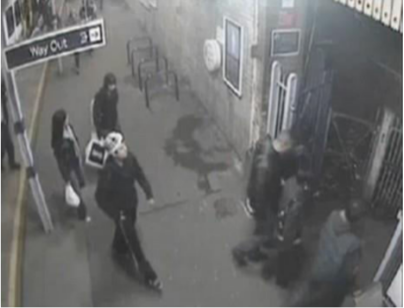
\includegraphics[scale = 0.6]{occlusion.png}
\caption{Occlusion Problem}
\end{figure}
Crowd scenes contain some uncertainities such as change of density, shape,
boundaries of the crowd. They do not define how to behave or share clear expectations
14on what will happen. They often feel something must be done right away to address
their common concern. Attitudes and ideas about the common concern spread very
quickly among crowd members. They often do and say things that they would normally
not do, and they go along with the actions of others in the crowd.\par
Certain crowd behaviours are normal in one scenario but may become hazards in
another. For example if we consider the running activity, running in a marathon can be
considered as a normal crowd behaviour but whereas running in a shopping mall or any
such rare places can be considered as an abnormal behaviour.
\begin{figure}[H]
\centering
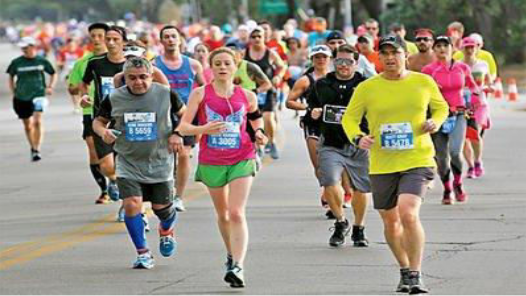
\includegraphics[scale = 0.7]{crowd_marathon.png}
\caption{Crowd Running in Marathon}
\end{figure}
\begin{figure}[H]
\centering
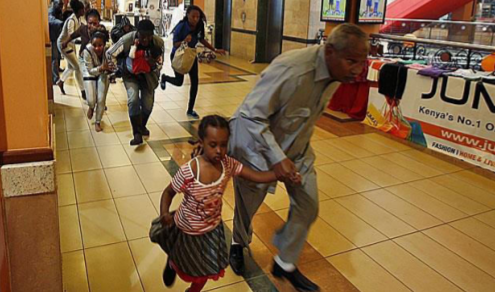
\includegraphics[scale = 0.7]{crowd_panic_mall.png}
\caption{Crowd Running in a Mall}
\end{figure}
\section{Optical Flow}
\subsection{What is Optical Flow}
Optical flow or optic flow is the pattern of apparent motion of objects, surfaces,
and edges in a visual scene caused by the relative motion between an observer and a
scene. The concept of optical flow was introduced by the American psychologist James
J. Gibson in the 1940s to describe the visual stimulus provided to animals moving
through the world. Gibson stressed the importance of optic flow for affordance
perception, the ability to discern possibilities for action within the environment.\par
Followers of Gibson and his ecological approach to psychology have further demonstrated the role of the optical flow stimulus for the perception of movement by
the observer in the world; perception of the shape, distance and movement of objects in
the world; and the control of locomotion.
The term optical flow is also used by roboticists, encompassing related
techniques from image processing and control of navigation including motion detection,
object segmentation, time-to-contact information, focus of expansion calculations,
luminance, motion compensated encoding, and stereo disparity measurement.

\subsection{Estimation}
Sequences of ordered images allow the estimation of motion as either
instantaneous image velocities or discrete image displacements. Fleet and Weiss
provide a tutorial introduction to gradient based optical flow. John L. Barron, David J.
Fleet, and Steven Beauchemin provide a performance analysis of a number of optical
flow techniques. It emphasizes the accuracy and density of measurements.\par
The optical flow methods try to calculate the motion between two image frames
which are taken at consecutive time frames at every voxel position. These methods are
called differential since they are based on local Taylor series approximations of the
image signal; that is, they use partial derivatives with respect to the spatial and temporal
coordinates. \par
For a 2D+t dimensional case (3D or n-D cases are similar) a voxel at location (x,y,t)
with intensity I(x,y,t) will have moved between the two image frames, and the following
brightness constancy constraint can be given:
\begin{equation}
I(x,y,t) = T(x + \Delta x, y + \Delta y, t + \Delta t)
\end{equation}
\begin{equation}
\frac{\partial I}{\partial x}V_x + \frac{\partial I}{\partial y}V_y + \frac{\partial I}{\partial t} = 0
\end{equation}
\chapter{Requirements, Analysis and Specifications}
\section{Unix}
Unix is a family of multitasking, multiuser computer operating systems that derive from the original AT\&T Unix, development starting in the 1970s at the Bell Labs research center by Ken Thompson, Dennis Ritchie, and others.
Unix was originally meant to be a convenient platform for programmers developing software to be run on it and on other systems, rather than for non-programmers. The system grew larger as the operating system started spreading in academic circles, as users added their own tools to the system and shared them with colleagues.
\begin{itemize}
	\item Kernel - source code in /usr/sys, composed of several sub-components.
	\item Development environment – early versions of Unix contained a development environment sufficient to recreate the entire system from source code.
	\item Commands – Unix makes little distinction between commands (user-level programs) for system operation and maintenance (e.g. cron), commands of general utility (e.g. grep), and more general-purpose applications such as the text formatting and typesetting package. Nonetheless, some major categories are.
	\item Document formatting – Unix systems were used from the outset for document preparation and typesetting systems, and included many related programs such as nroff, troff, tbl, eqn, refer, and pic. Some modern Unix systems also include packages such as TeX and Ghostscript.
	\item Graphics – the plot subsystem provided facilities for producing simple vector plots in a device-independent format, with device-specific interpreters to display such files. Modern Unix systems also generally include X11 as a standard windowing system and GUI, and many support OpenGL.
	\item Communications – early Unix systems contained no inter-system communication, but did include the inter-user communication programs mail and write. V7 introduced the early inter-system communication system UUCP, and systems beginning with BSD release 4.1c included TCP/IP utilities.
\end{itemize}
\section{Python}
Only open source languages and tools are used in developing the project. Unix environment is being used for the development of the process.
Language used is Python and the main tool used is OpenCV for video processing. Python is interpreted language which is used for general-purpose programming. It is a user-friendly language which emphasizes on code readability and its syntax allows users to write programs with relatively fewer lines of code when compared to C/C++, Java etc. Python 2.7 version is used in the project.\\
Python's \textbf{features} include:
\begin{itemize}
\item Easy-to-learn: Python has few keywords, simple structure, and a clearly defined syntax. This allows the student to pick up the language quickly.
\item Easy-to-read: Python code is more clearly defined and visible to the eyes.
\item Easy-to-maintain: Python's source code is fairly easy-to-maintain.
\item A broad standard library: Python's bulk of the library is very portable and cross-platform compatible on UNIX, Windows, and Macintosh.
\item Interactive Mode: Python has support for an interactive mode which allows interactive testing and debugging of snippets of code.
\item Portable: Python can run on a wide variety of hardware platforms and has the same interface on all platforms.
\item Extendable: You can add low-level modules to the Python interpreter. These modules enable programmers to add to or customize their tools to be more efficient.
\item Databases: Python provides interfaces to all major commercial databases.
\item GUI Programming: Python supports GUI applications that can be created and ported to many system calls, libraries and windows systems, such as Windows MFC, Macintosh, and the X Window system of Unix.
\item Scalable: Python provides a better structure and support for large programs than shell scripting.
\end{itemize}
Apart from the above-mentioned features, Python has a big list of good features, few are listed below:
\begin{itemize}
	\item It supports functional and structured programming methods as well as OOP.
\item It can be used as a scripting language or can be compiled to byte-code for building large applications.
\item It provides very high-level dynamic data types and supports dynamic type checking.
\item It supports automatic garbage collection.
\item It can be easily integrated with C, C++, COM, ActiveX, CORBA, and Java.

\end{itemize}
\section{OpenCV}
OpenCV (Open Source Computer Vision Library) is an open source computer vision and machine learning software library. OpenCV was built to provide a common infrastructure for computer vision applications and to accelerate the use of machine perception in the commercial products. Being a BSD-licensed product, OpenCV makes it easy for businesses to utilize and modify the code.\par
The library has more than 2500 optimized algorithms, which includes a comprehensive set of both classic and state-of-the-art computer vision and machine learning algorithms. These algorithms can be used to detect and recognize faces, identify objects, classify human actions in videos, track camera movements, track moving objects, extract 3D models of objects, produce 3D point clouds from stereo cameras, stitch images together to produce a high resolution image of an entire scene, find similar images from an image database, remove red eyes from images taken using flash, follow eye movements, recognize scenery and establish markers to overlay it with augmented reality, etc. OpenCV has more than 47 thousand people of user community and estimated number of downloads exceeding 14 million. The library is used extensively in companies, research groups and by governmental bodies.\par
Along with well-established companies like Google, Yahoo, Microsoft, Intel, IBM, Sony, Honda, Toyota that employ the library, there are many start-ups such as Applied Minds, VideoSurf, and Zeitera, that make extensive use of OpenCV. OpenCV’s deployed uses span the range from stitching street view images together, detecting intrusions in surveillance video in Israel, monitoring mine equipment in China, helping robots navigate and pick up objects at Willow Garage, detection of swimming pool drowning accidents in Europe, running interactive art in Spain and New York, checking runways for debris in Turkey, inspecting labels on products in factories around the world on to rapid face detection in Japan.\par
OpenCV is written in C++ and its primary interface is in C++, but it still retains a less comprehensive though extensive older C interface. There are bindings in Python, Java and MATLAB/OCTAVE. The API for these interfaces	can be found in the online documentation. Wrappers in other languages such as C-sharp, Perl, Ch, Haskell and Ruby have been developed to encourage adoption by a wider audience. All the new developments and algorithms in OpenCV are now developed in the C++ interface.\\
There are many \textbf{applications} of OpenCV. A few of them are cited as below:
\begin{itemize}
\item 2D and 3D feature toolkits 
\item Facial recognition system 
\item Gesture recognition 
\item Human–computer interaction (HCI) 
\item Mobile robotics 
\item Motion understanding 
\item Object identification 
\item Segmentation and recognition 
\item Stereopsis stereo vision: depth perception from 2 cameras 
\item Structure from motion (SFM) 
\item Motion tracking 
\end{itemize}
\section{Hardware Requirements}
\begin{itemize}
	\item Processor - Intel Core i5 5th gen
	\item RAM - 8 GB
	\item Hard Disk - 500 GB
	\item OS - Unix based such as Debian , MacOS
	\item WebCam
	\item USB 2.0 Ports
\end{itemize}
\section{Others}
\subsection{Libraries}
Along with OpenCV we have used bob. Bob is a machine learning platform used in python, it helped us to port Matlab code of optical flow to python. Scikit learn is Python package which is similar to WEKA tool for java. It will be used for training a classifier model in the proposed algorithm of the project.

\subsection{Editor}
An editor is required to create python source files and to view violent features generated for the dataset. Open source editors like Atom and PyCharm have been used which also provide terminal access.

\subsection{Video Player}
To play all the videos through openCV and to view some random videos. Video players like VLC is required which is open source. ffmpeg library is also required which provides a way to read video files through openCV. ffmpeg can also be used to format videos.
\chapter{Methodology}
\section{System Design}
The project focuses on the implementation of an algorithm that can detect disturbance in crowd. It considers how flow-vector magnitudes change over time, which are collected for short frame sequences, and then classified as either normal or abnormal situation using a classifier.
\par
The aim of the project is to keep the processing very quick, a detection should be made within a few seconds of the outbreak of violence. It has to detect the change of normal behaviour to abnormal behaviour with the shortest delay from the time that the change has occurred.

\begin{figure}[H]
\centering
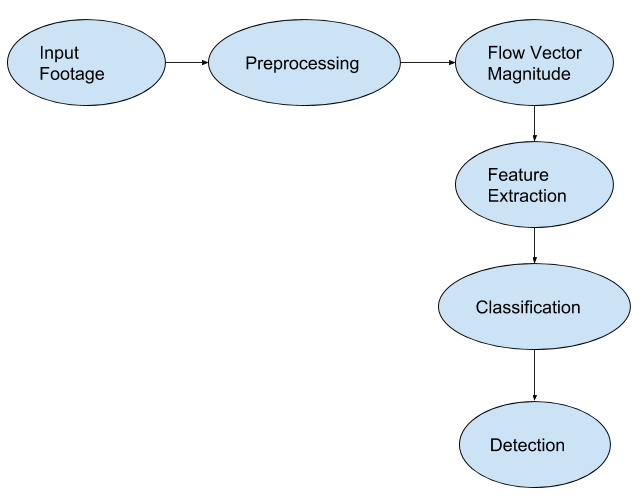
\includegraphics[scale = 0.4]{system_design.png}
\caption{System Design}
\end{figure}

\section{Implementation of Proposed Solution}
\subsection{Input Footage}
For training of the classifier input of the footage will be from a fixed dataset. For practical real time implementation footage from externally attached cameras can be used. The resolution of the input footage need not be specific. Generally the resolution of a CCTV footage is of 704 X 480 pixels. This proposed algorithm reduces the height of the video to 100 pixels and width accordingly. This increases the scalability of the algorithm. Even high definition videos can be processed with the proposed algorithm.
\subsection{Preprocessing}
Preprocessing the input data is very important part of the algorithm. Optical flow algorithm will take at least one minute to calculate optical flow of a high definition image. So as to constraint the processing to real time preprocessing must done. As mentioned earlier any image is being resized to 100 pixel height and respective width accordingly. Preprocessing is done in a way such that the aspect ratio of the video is not disturbed.
\subsection{Flow Vector Magnitude}
For each pixel in the video has some velocity corresponding to it, along x direction and y direction. The Flow Vector Magnitude is nothing but the magnitudes of these velocities. Computing Flow Vector Magnitude is computationally heavy, this is the most time taking part of the proposed algorithm. Since we are reducing the size of frames considerably, this is computation is quick enough to cope us with real time violence detection.
\subsection{Feature Extraction}
Feature extraction is based on the computation of ViF (Violence Flow Descriptors). These descriptors are quantised values of the above generated Flow Vector Magnitudes. After ViF is generated a histogram is built which will assign different ViF values to corresponding bins in the range of (0 to 1.0) with the intervals of 0.05, i.e 20 bins.
\subsection{Classification}
After the features have been extracted, classification can done with the help of a simple Linear SVM. So as to further increase the accuracy of the algorithm , SVM with AdaBoost can be used. For our project a trained neural net has been used since it is providing a better accuracy.
\subsection{Detection}
Detection in a video footage is the final output of the proposed algorithm. It is taking place with the help classifier model that is being trained in the above step. According to the base paper, a sequence of 10 frames i.e on an average two-fifth of a second is enough to detect violence in a footage. Detection may be further improved continuous learning in real-time also.
\section{Languages and Tools}
Only open source languages and tools are used in developing the project. Unix environment is being used for the development of the process.
\subsection{Language}
Language used is Python and the main tool used is OpenCV for video processing. Python is interpreted language which is used for general-purpose programming. It is a user-friendly language which emphasizes on code readability and its syntax allows users to write programs with relatively fewer lines of code when compared to C/C++, Java etc. Python 2.7 version is used in the project.\\
Python's \textbf{features} include:
\begin{itemize}
\item Easy-to-learn: Python has few keywords, simple structure, and a clearly defined syntax. This allows the student to pick up the language quickly.
\item Easy-to-read: Python code is more clearly defined and visible to the eyes.
\item Easy-to-maintain: Python's source code is fairly easy-to-maintain.
\item A broad standard library: Python's bulk of the library is very portable and cross-platform compatible on UNIX, Windows, and Macintosh.
\item Interactive Mode: Python has support for an interactive mode which allows interactive testing and debugging of snippets of code.
\item Portable: Python can run on a wide variety of hardware platforms and has the same interface on all platforms.
\item Extendable: You can add low-level modules to the Python interpreter. These modules enable programmers to add to or customize their tools to be more efficient.
\item Databases: Python provides interfaces to all major commercial databases.
\item GUI Programming: Python supports GUI applications that can be created and ported to many system calls, libraries and windows systems, such as Windows MFC, Macintosh, and the X Window system of Unix.
\item Scalable: Python provides a better structure and support for large programs than shell scripting.
\end{itemize}
Apart from the above-mentioned features, Python has a big list of good features, few are listed below:
\begin{itemize}
	\item It supports functional and structured programming methods as well as OOP.
\item It can be used as a scripting language or can be compiled to byte-code for building large applications.
\item It provides very high-level dynamic data types and supports dynamic type checking.
\item It supports automatic garbage collection.
\item It can be easily integrated with C, C++, COM, ActiveX, CORBA, and Java.

\end{itemize}
\subsection{OpenCV}
OpenCV (Open Source Computer Vision Library) is an open source computer vision and machine learning software library. OpenCV was built to provide a common infrastructure for computer vision applications and to accelerate the use of machine perception in the commercial products. Being a BSD-licensed product, OpenCV makes it easy for businesses to utilize and modify the code.\par
The library has more than 2500 optimized algorithms, which includes a comprehensive set of both classic and state-of-the-art computer vision and machine learning algorithms. These algorithms can be used to detect and recognize faces, identify objects, classify human actions in videos, track camera movements, track moving objects, extract 3D models of objects, produce 3D point clouds from stereo cameras, stitch images together to produce a high resolution image of an entire scene, find similar images from an image database, remove red eyes from images taken using flash, follow eye movements, recognize scenery and establish markers to overlay it with augmented reality, etc. OpenCV has more than 47 thousand people of user community and estimated number of downloads exceeding 14 million. The library is used extensively in companies, research groups and by governmental bodies.\par
Along with well-established companies like Google, Yahoo, Microsoft, Intel, IBM, Sony, Honda, Toyota that employ the library, there are many start-ups such as Applied Minds, VideoSurf, and Zeitera, that make extensive use of OpenCV. OpenCV’s deployed uses span the range from stitching street view images together, detecting intrusions in surveillance video in Israel, monitoring mine equipment in China, helping robots navigate and pick up objects at Willow Garage, detection of swimming pool drowning accidents in Europe, running interactive art in Spain and New York, checking runways for debris in Turkey, inspecting labels on products in factories around the world on to rapid face detection in Japan.\par
OpenCV is written in C++ and its primary interface is in C++, but it still retains a less comprehensive though extensive older C interface. There are bindings in Python, Java and MATLAB/OCTAVE. The API for these interfaces	can be found in the online documentation. Wrappers in other languages such as C-sharp, Perl, Ch, Haskell and Ruby have been developed to encourage adoption by a wider audience. All the new developments and algorithms in OpenCV are now developed in the C++ interface.\\
There are many \textbf{applications} of OpenCV. A few of them are cited as below:
\begin{itemize}
\item 2D and 3D feature toolkits 
\item Facial recognition system 
\item Gesture recognition 
\item Human–computer interaction (HCI) 
\item Mobile robotics 
\item Motion understanding 
\item Object identification 
\item Segmentation and recognition 
\item Stereopsis stereo vision: depth perception from 2 cameras 
\item Structure from motion (SFM) 
\item Motion tracking 
\end{itemize}

\subsection{Other libraries}
Along with OpenCV we have used bob. Bob is a machine learning platform used in python, it helped us to port Matlab code of optical flow to python. Scikit learn is Python package which is similar to WEKA tool for java. It will be used for training a classifier model in the proposed algorithm of the project.



\chapter{Dataset}
In-the-wild violence dataset is chosen as dataset for the project. The dataset consists of 246 videos in which half are violent and other half are non-violent. The video duration range from 1.04 sec to 6.52 sec with an average duration of 3.60 sec. All the videos are downloaded from YouTube which are produced under in-the-wild and uncontrolled conditions presenting a wide range of real-world viewing conditions, video qualities and surveillance scenarios. Videos are compressed using the DivX codec (mpeg4) and resized to 240 X 320 pixels.

\begin{center}
\begin{figure}[H]
\centering
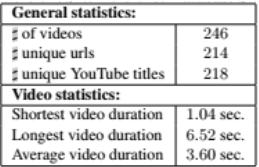
\includegraphics{dataset.png}
\caption{Dataset}
\end{figure}
\end{center}
\chapter{Design}
\section{Data Flow Diagram}
A data flow diagram is a graphical representation of the "flow" of data through an information system, modelling its process aspects. A DFD is often used as a preliminary step to create an overview of the system without going into great detail, which can later be elaborated. DFD's can be used for the visualization of data processing.
\par
Data flow diagrams are also known as bubble charts. DFD is a designing tool used in the top-down approach to system design. This context-level DFD is next "exploded", to produce a level-1 DFD that shows some of the detail of the system being modeled. The Level-1 DFD shows how the system is divided into subsystems, each of which deals with one or more of the data flows to from an external agent, and which together provide all of the functionality of the system as a whole. It also identifies internal data stores that must be present in order for the system to do its job, and shows the flow of data between the various parts of the system.

\begin{center}
\begin{figure}[H]
\centering
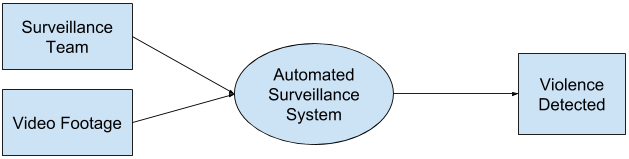
\includegraphics[width = \linewidth]{dfd0.png}
\caption{Data Flow Diagram Level 0}
\end{figure}
\end{center}

\begin{center}
\begin{figure}[H]
\centering
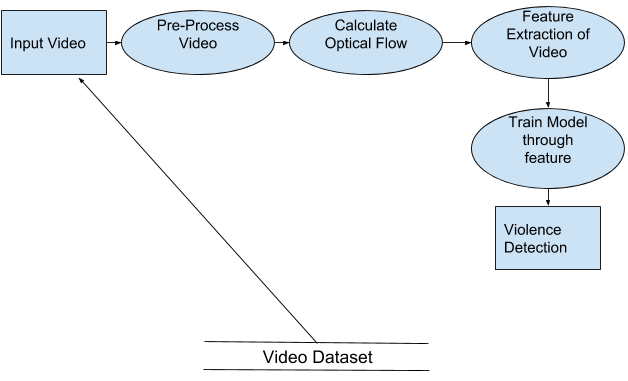
\includegraphics[width = \linewidth]{dfd1.png}
\caption{Data Flow Diagram Level 1}
\end{figure}
\end{center}

\section{UML Diagrams}
UML stands for Unified Modeling Language. UML is a standardized general-purpose modeling language in the field of object-oriented software engineering. The standard is managed, and was created by, the Object Management Group. 
\par
The UML is a very important part of developing objects oriented software and the software development process. The UML uses mostly graphical notations to express the design of software projects.\\
\subsection{Building blocks of UML}
The vocabulary of the UML encompasses three kinds of building blocks.
\begin{enumerate}
	\item Things.
	\item Relationships.
	\item Diagrams.
\end{enumerate}
\subsection{Things in UML}
Things are the abstractions that are first-class citizen in a model.\\
There are four kinds of things in the UML.
\begin{enumerate}
	\item Structure things.
	\item Behavioural things.
	\item Grouping things.
	\item Annotational things.
\end{enumerate}
These things are the basic object-oriented building blocks of the UML. You use them to write well-formed models.
\subsection{Relationships in the UML}
Things can be connected to logically be physically with the help of relationship in object oriented modelling.These are four kinds of relationships in the UML.

\begin{enumerate}
	\item Dependency.
	\item Association.
	\item Generalization.
	\item Realization.
\end{enumerate}
\subsection{Diagrams in UML}
A diagram is a graphical representation of a set of elements. These are nine kinds of diagrams in the UML.
\begin{enumerate}
	\item Class diagram.                 
\item  Object diagram                
\item  Use Case diagram.               
\item  Sequence diagram.             
\item  Collaboration diagram.
\item  Activity diagram.
\item  Component diagram.
\item  State chart diagram.
\item  Deployment diagram.

\end{enumerate}
\subsection{Component Diagram}
Automated Surveillance and Alert Generation System has the following components:
\begin{enumerate}
	\item OpenCV
	\item Bob
	\item Video Preprocess
	\item Optical Flow
	\item Violent Feature Extract
\end{enumerate}
\begin{center}
\begin{figure}[H]
\centering
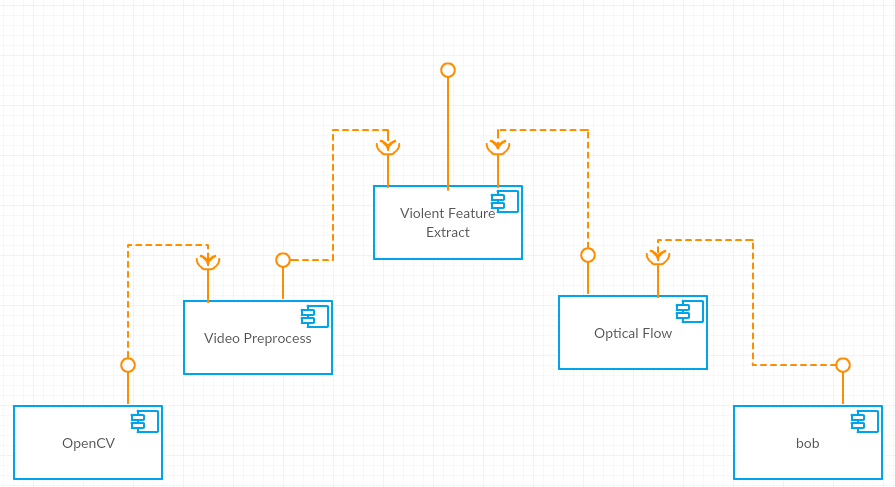
\includegraphics[width = \linewidth]{component.png}
\caption{Component Diagram}
\end{figure}
\end{center}
\subsubsection{OpenCV}
OpenCV (short for Open Computer Vision) is a package originally written in C language but later it was ported to Python. OpenCV possesses a rich set of interfaces and functions  that help us to read and manipulate video files. OpenCV can read video from input cameras and also from attached cameras to the system. Given a source of CCTV footage , through OpenCV we are able to manipulate frame size, the colour and the frame intervals. Video Preprocessing has to be done so that the further components can work at real-time which is on and average 1/25 th of a second for a frame.
\subsubsection{Bob}
Bob is a signal processing and machine learning platform available for python. Bob is provided as a precompiled source for Linux or Mac OS through Anaconda package manager. Bob helps us to port the signal processing procedures which are initially written in C language. Signal processing methods are usually written in C language as it can make native function calls and kernel function calls. So as to port these procedures into Python bob platform is used. C Liu’s Optical Flow algorithm [5] is being ported here through bob.
\subsubsection{Video Preprocess}
This is a self written Python library. It Preprocesses the video according to our needs. This library makes the necessary calls from the OpenCV so as to do the pixel level manipulations. Frame by Frame access is done by through this package. Frame interval is set as 3, default frame rate is taken as 25, each frame is resized to 100 pixel width and corresponding height. Frame is further converted into grayscale.
\subsubsection{Optical Flow}
This is also a self written package. It contains the procedures to calculate Optical flow which further call procedures from bob platform. Optical flow will return 3 things in a tuple, velocity along x , y axis and the wrap. This calculation is done by considering some pre calculated parameters.
\subsubsection{Video Feature Extract}
At a considered moment, three frames are under consideration. Previous frame , current frame and the next frame. First thing we do is we preprocess these frames and then calculated optical flows between successive frames. Now we have two optical flow vectors, now we calculate the absolute change between these two vectors. Average of this change vector is calculated and it is stored as threshold. Now the change vector is quantised with binary 1 and 0 by comparing it with threshold vector. This binary vector is summed for the whole video and normalized by dividing it with the number of iterations done till now. Binary vector generated till now is divided into (4 * 4) parts. For each of these parts , a histogram is built which has the bin size of 0.05 ranging from 0 to 1. Frequency of each bin is calculated and normalized by dividing with sum of all frequencies. Now all of the normalized histograms are appended one after another and the resulting vector is known as \textit{Violent Feature Vector}.
\chapter{Implementation}
\section{Video Preprocessing}
Surveillance footage is usually generated of size 240 x 320 i.e of aspect ratio of 3:4. Considered video format is of avi. If the video is not present in the given format, we use the ffmpeg command to convert the video to the required format. 
\\
Video conversion command:-\\
\textit{ffmpeg -i {inputVideo} -vf scale=320:240 outputVideo.avi}
\par
Further the frame is resized to 75 x 100 size maintaining the same aspect ratio using openCV functions. This resized frame is further converted to grayscale using openCV cvtColor method. \\
Size reduction command:\\
frame = cv2.resize(frame, dim, interpolation = cv2.INTER\_AREA)\\
Grayscale conversion commands: \\
frame = cv2.cvtColor(frame,cv2.COLOR\_BGR2GRAY)
\begin{center}
\begin{figure}[H]
\centering
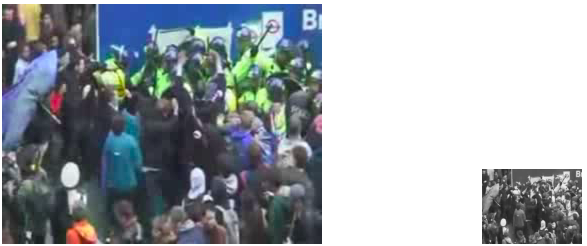
\includegraphics[width = \linewidth]{frame_resize.png}
\caption{Frames before and after preprocessing respectively}
\end{figure}
\end{center}
\section{Optical Flow}
Optical Flow is estimated between the pair of consecutive frames which gives a flow vector for each pixel in the current frame, matching it to pixel in next frame. C. Liu’s Optical Flow algorithm is used. It was initially developed in C++ which MATLAB can easily port. Conda package was used to port the algorithm into Python. \par
	In our implementation we are considering two frames in every four frames i.e the third frame from current frame and calculating optical flow between them. This process continues for entire video. \par \textbf{bob.ip.optflow.liu.sor.flow(frame1,frame2)} is used to calculate optical flow. It returns value of each pixel into a numpy array of dimension equal to resolution of the frame.
\begin{center}
\begin{figure}[H]
\centering
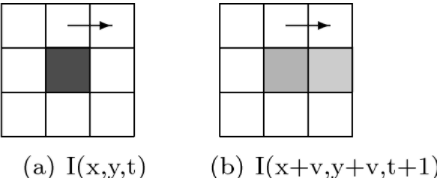
\includegraphics[width = \linewidth]{optical_flow.png}
\caption{Example Optical Flow}
\end{figure}
\end{center}

\section{Violent Features}
Once the optical flow has been generated, flow vector magnitude is calculated through the following formula:- \\
$ m_{x,y,t} = \sqrt{V_{x,t}^2 + V_{y,t}^2} $ \\
\par
After calculating flow vector , for each pixel in each frame we obtain the binary indicators using the following formula:- \\
\begin{equation}
b_{x,y,t} = \begin{cases}
\text {1,\quad}if\quad |m_{x,y,t+1} - m_{x,y,t-1}| \geq \theta\\
\text {0\quad}   \quad otherwise
\end{cases}
\end{equation}
\par
Next we calculate the mean magnitude change by simply averaging these binary indicators for each frame:- 
\begin{equation}
\overline b_{x,y} = \frac{1}{T}\sum_{t}b_{x,y,t}
\end{equation}
\par
This average binary vector obtained is known as Violent Flow Descriptor (ViF). This ViF values is used for further training and classifications purposes.
	After ViF’s are obtained for a video, a histogram in created of bin size 0.05 and from range 0.0 to 1.0. Which means 21 bins are created. Generated ViF is divided into 16 parts, each part is mapped into a separate histogram, the counts are further normalized by total counts obtained. This process is known as Histogram normalization. Now all these histogram bins values for all 16 parts are appended one after the other leading to generation 336 values for a particular video. 
These 336 values are used for training the neural net and for predicting using the neural net.
\section{Training Neural Net}
Keras module along with TensorFlow backend is used to build the Neural Net and Train it. The Neural Net built contains an Input Layer, two Dense Layers and an Output Layer. Each layer is of 336 nodes. Input to the neural net will the Violent Flow Features(ViF) which is a numpy array of dimensions 129*336. Activation function for Input and Middle Layers is ReLU(Rectifier Linear Unit) and for output layer, Sigmoid activation function is used. Training is done for 150 epochs with batch size of 10. Outputs will in the range of 0.0 to 1.0 which will rounded off accordingly. \\
ReLU activation Function \\
f(x) = max(0,x)\\
Sigmoid activation function \\
S(x) = $\frac{1}{1+e^{-x}} = \frac{e^x}{1+e^x}$
\begin{center}
\begin{figure}[H]
\centering
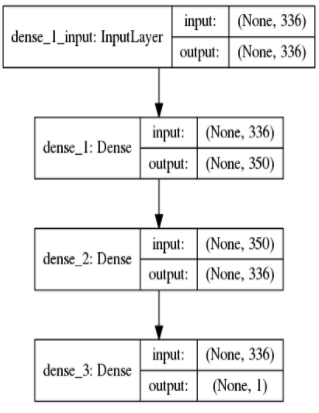
\includegraphics[scale = 0.6]{neural_net.png}
\caption{Neural Net Layer Information}
\end{figure}
\end{center}
\section{Violence Detection}
Keras module has been used to train the neural network. The average FPS rate of a video is to be considered 30fps. Average surveillance videos have an FPS rate of 30fps. We consider every 3rd frame for calculating ViF’s. 
\par
	Every 30 frames , i.e every 1 second 336 length array is generated and that array is sent to the previously generated model for prediction. If violence is detected, violence probability is shown on the screen. Multiple lengthy videos have been given an input to the program and it is able to detect the instance where crowd behaviour tends to violent from non\_violent.



\clearpage
\chapter{Results}
The following partial results will be present in the further sections:
\begin{itemize}
	\item Video Preprocessing
	\item Optical Flow
	\item Violent Features
	\item Neural Net N-Folds accuracy
	\item Real Time Surveillance on Video
	\item Real Time Surveillance on Camera Input
\end{itemize}
\section{Video Preprocessing}
 Input frames are resized to 240 X 320. They are further converted to grayscale.
\begin{center}
\begin{figure}[H]
\centering
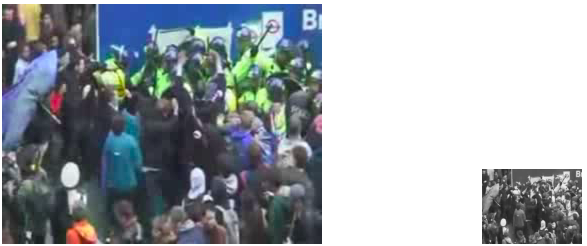
\includegraphics[width = \linewidth]{frame_resize.png}
\caption{Frames before and after preprocessing}
\end{figure}
\end{center}
\section{Optical Flow}
Optical flow refers to the visible motion of an object in an image, and the apparent 'flow' of pixels in an image. It is the result of 3d motion being projected on a 2-d image plane. 
\begin{figure}[htp]
\centering
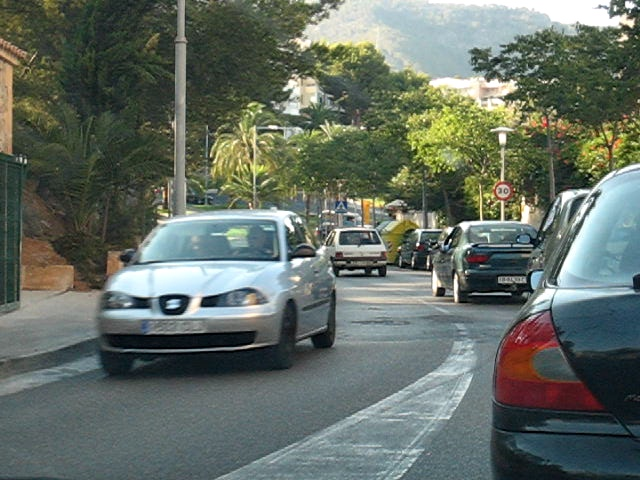
\includegraphics[width=.3\textwidth]{car1.jpg}\hfill
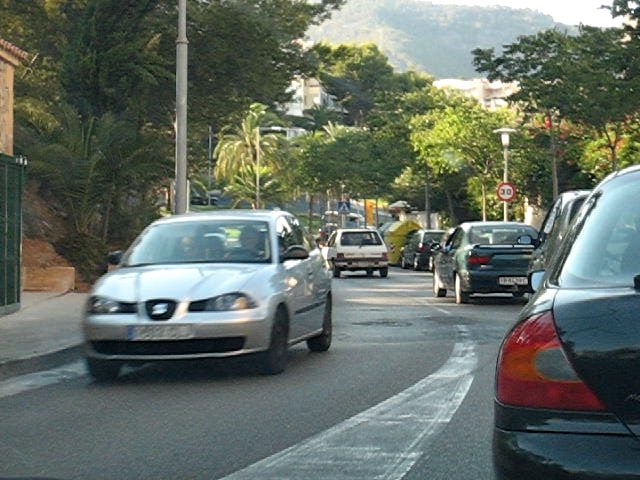
\includegraphics[width=.3\textwidth]{car2.jpg}\hfill
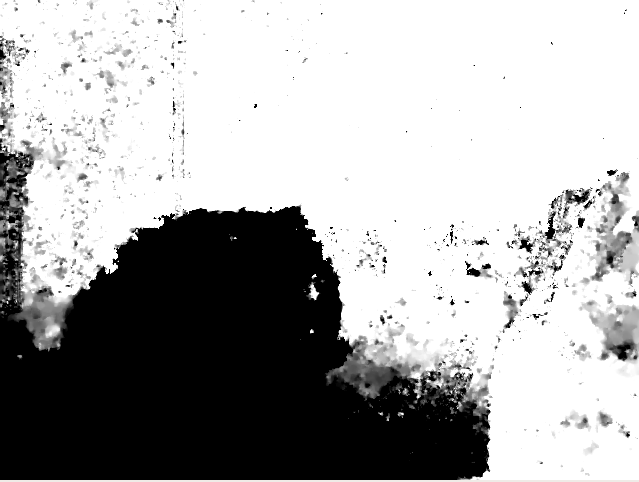
\includegraphics[width=.3\textwidth]{car_opt_flow.png}
\caption{Optical Flow Car Example}
\end{figure}
\section{Violent Features}
Violent Features for a video will contains 336 features. There are 21 bins in a histogram and each frame is divided into 16 blocks. Hence it results into a total of 21 * 16 = 336 features ranging from 0.0 to 1.0 .
\lstset{
  basicstyle=\ttfamily,
  columns=fullflexible,
  frame=single,
  breaklines=true,
  postbreak=\mbox{\textcolor{red}{$\hookrightarrow$}\space},
}
\definecolor{Code}{rgb}{0,0,0}
\definecolor{Decorators}{rgb}{0.5,0.5,0.5}
\definecolor{Numbers}{rgb}{0.5,0,0}
\definecolor{MatchingBrackets}{rgb}{0.25,0.5,0.5}
\definecolor{Keywords}{rgb}{0,0,1}
\definecolor{self}{rgb}{0,0,0}
\definecolor{Strings}{rgb}{0,0.63,0}
\definecolor{Comments}{rgb}{0,0.63,1}
\definecolor{Backquotes}{rgb}{0,0,0}
\definecolor{Classname}{rgb}{0,0,0}
\definecolor{FunctionName}{rgb}{0,0,0}
\definecolor{Operators}{rgb}{0,0,0}
\definecolor{Background}{rgb}{0.98,0.98,0.98}
\lstdefinelanguage{Python}{
numbers=left,
numberstyle=\footnotesize,
numbersep=1em,
xleftmargin=1em,
framextopmargin=2em,
framexbottommargin=2em,
showspaces=false,
showtabs=false,
showstringspaces=false,
frame=l,
tabsize=4,
% Basic
basicstyle=\ttfamily\small\setstretch{1},
backgroundcolor=\color{Background},
% Comments
commentstyle=\color{Comments}\slshape,
% Strings
stringstyle=\color{Strings},
morecomment=[s][\color{Strings}]{"""}{"""},
morecomment=[s][\color{Strings}]{'''}{'''},
% keywords
morekeywords={import,from,class,def,for,while,if,is,in,elif,else,not,and,or,print,break,continue,return,True,False,None,access,as,,del,except,exec,finally,global,import,lambda,pass,print,raise,try,assert},
keywordstyle={\color{Keywords}\bfseries},
% additional keywords
morekeywords={[2]@invariant,pylab,numpy,np,scipy},
keywordstyle={[2]\color{Decorators}\slshape},
emph={self},
emphstyle={\color{self}\slshape},
%
}
\linespread{1.3}\\
\textbf{Sample Vif}
\lstinputlisting[language = Python]{sample_vif.txt}

\section{Neural Net N-folds Cross Verification}
Seven fold cross validation is the validation manner which is adopted in
experiments. All the videos are divided into seven heaps with the same ratio between
violent and non-violent ones. At each time one distinct heap is selected for testing and the other six heaps for training. This procedure is then repeated for seven times.
\begin{figure}[H]
\centering
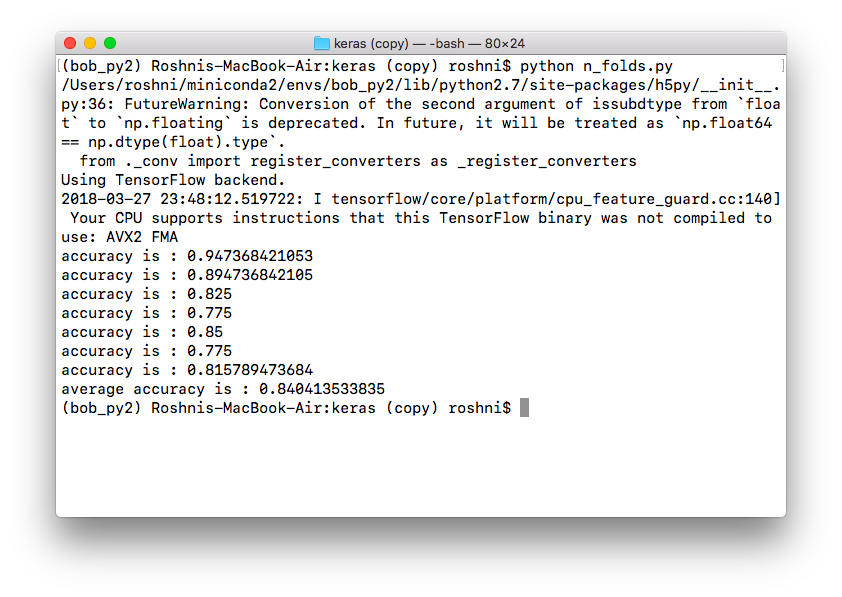
\includegraphics[width = \linewidth]{84_nfolds_keras.png}
\caption{Neural Net Folds Accuracy}
\end{figure}
\section{Real Time Surveillance on Video Input}
There usually FPS rate of a standard surveillance is 25. Which means our algorithm has to process each frame in less than 1/25 th of a second. Real Time Surveillance of a Video outputs on terminal and it provides the exact second where the frames go from violent to non-violent. So with the help of this we are able to decide the exact second where the violence occurs. 
\begin{figure}[H]
\centering
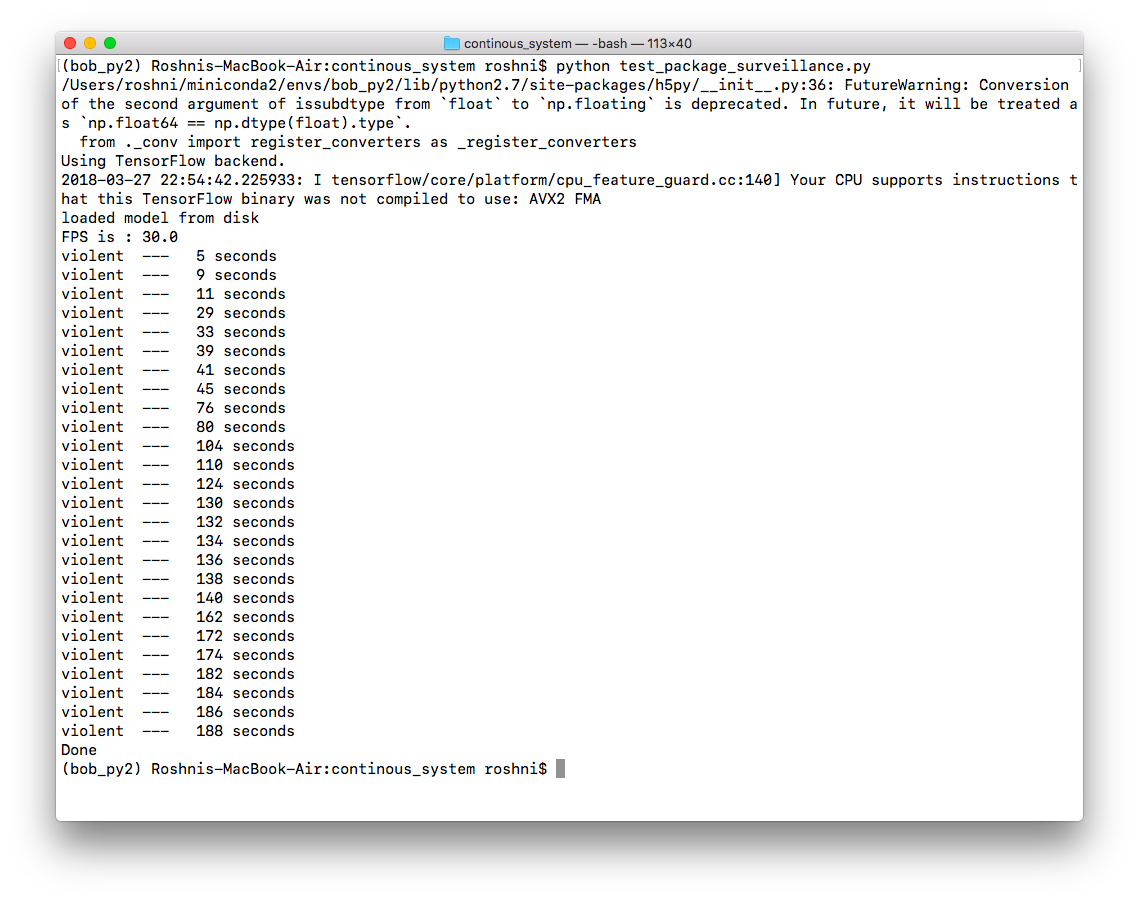
\includegraphics[width = \linewidth]{video_surveillance_output.png}
\caption{Surveillance on Video}
\end{figure}
\section{Real Time Surveillance on Camera Input}
OpenCV helps us to take video input directly from the camera connected. It can be externally connected through a usb port or it can be the internal webcam.
\begin{figure}[H]
\centering
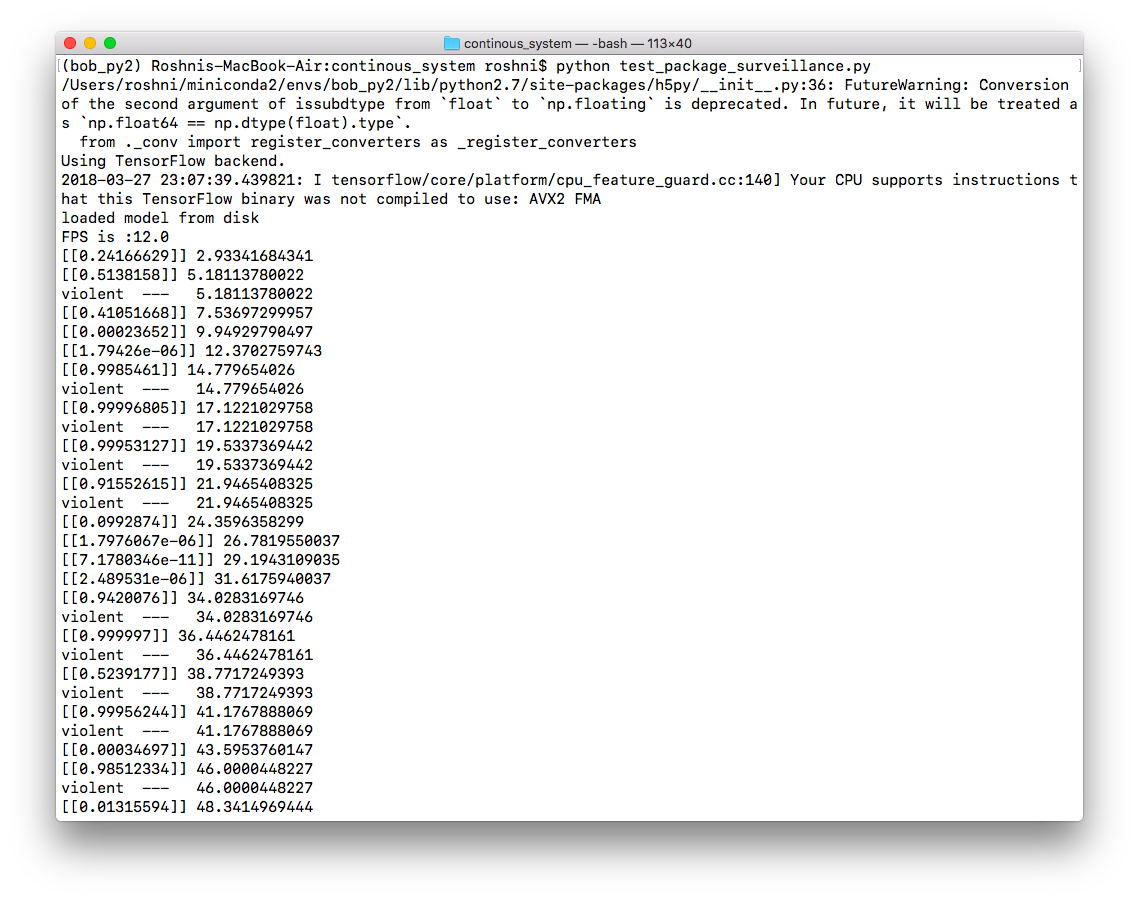
\includegraphics[width = \linewidth]{camera_surveillance_output.png}
\caption{Surveillance through Camera}
\end{figure}
\section{Result Ananlysis}
\begin{longtable}{|p{3cm}|p{3cm}|p{2cm}|p{4cm}|p{3cm}|}
\hline
\textbf{Title} & \textbf{Methodology} & \textbf{Results} & \textbf{Merits}  & \textbf{Demerits}\\
\hline
\endhead
Violence detection using Oriented Violent Flows, 2016 [1] & AdaBoost and SVM classifier. & 88.00 percent & Feature representation model, which depicts the information involving both the motion magnitude and motion orientation. & Detection point where the behaviour is changing from normal to abnormal is time consuming hence not applicable in real time scenerios.\\
\hline
Violent Flows:Real-Time Detection of Violent Crowd Behaviour, 2012 [2] & Global descriptors and SVM classifier & 5-fold cross validation: 81.30 percent & The algorithm detected far more violent scenes correctly, compared to existing work. It was furthermore far faster to detect the violence, typically in less than a second from its outbreak & Only magnitude of the flow vectors is considered, but the direction is not.\\
\hline

Automatic Fight
Detection in
Surveillance
Videos, 2016 [3] & 
Motion magnitude,
motion acceleration
and strength of
motion region
relationship,
collectively known as
motion signals & 
10 fold cross
validation:
82.70 percent & 
Difference
between
stimulated
fights and real
fights.
Doesn’t rely
on high level
behaviour
recognition,
Thus applicable to Low quality videos. & 
 Less accuracy is
achieved when
testing with real
fight scenarios\\
\hline
Online real-time
crowd behaviour
detection in video
sequences, 2015 [4] & 
Instant entropy and
temporal occupancy
variation & 
96 percent & 
Works
without the
need of
training phase. &
 Computational
speed (FPS) is
varying for
different
datasets. Not robust with different types of data. Only able to give the percentage of violence. Not ideal for generating alerts. Crowded Scenes are considered as violent.\\
\hline
\pagebreak
Proposed Algorithm & Using Global Descriptors (ViFs) along with Neural Network to accurately predict disturbance in crowd. & 85.00 percent & Highly Scalable, can process multiple videos at a time using GPUs. Accuracy can be greatly imporved by increasing weights to well performing features. Input from human surveyor can continously train the model for better performance in future. & Only works for avi videos. High processor speeds are required. Neural Net initial training takes time. \\
\hline
\caption{Result Analysis}
\end{longtable}

\chapter{Future Work}

<Future work here>

\chapter{Conclusion}

<Conclusion here>

\cleardoublepage
%\pagebreak
\phantomsection
\addcontentsline{toc}{chapter}{References}
\begin{thebibliography}{99}

\bibitem{hassner}
T.~Hassner, Y.~Itcher, O.~Kliper~Gross. \emph{Violent Flows: Real-Time Detection of Violent Crowd Behavior},3rd IEEE International Workshop on Socially Intelligent Surveillance and Monitoring (SISM) at the IEEE Conf. on Computer Vision and Pattern Recognition (CVPR),June 2012

\bibitem{liu}
Ce.~Liu. \emph{Beyond Pixels: Exploring New Representations and Applications for Motion Analysis},Massachusetts Institute of Technology,Ph.D. Thesis,2009

\bibitem{bob}
Anjos, Andr\'e AND El Shafey, Laurent AND Wallace, Roy AND G\"unther, Manuel AND McCool, Christopher AND Marcel, S\'ebastien. \emph{Bob: a free signal processing and machine learning toolbox for researchers},20th ACM Conference on Multimedia Systems (ACMMM), Nara Japan, 2012s


\end{thebibliography}

\begin{appendices}
\chapter{Code}
\lstset{
  basicstyle=\ttfamily,
  columns=fullflexible,
  frame=single,
  breaklines=true,
  postbreak=\mbox{\textcolor{red}{$\hookrightarrow$}\space},
}
\definecolor{Code}{rgb}{0,0,0}
\definecolor{Decorators}{rgb}{0.5,0.5,0.5}
\definecolor{Numbers}{rgb}{0.5,0,0}
\definecolor{MatchingBrackets}{rgb}{0.25,0.5,0.5}
\definecolor{Keywords}{rgb}{0,0,1}
\definecolor{self}{rgb}{0,0,0}
\definecolor{Strings}{rgb}{0,0.63,0}
\definecolor{Comments}{rgb}{0,0.63,1}
\definecolor{Backquotes}{rgb}{0,0,0}
\definecolor{Classname}{rgb}{0,0,0}
\definecolor{FunctionName}{rgb}{0,0,0}
\definecolor{Operators}{rgb}{0,0,0}
\definecolor{Background}{rgb}{0.98,0.98,0.98}
\lstdefinelanguage{Python}{
numbers=left,
numberstyle=\footnotesize,
numbersep=1em,
xleftmargin=1em,
framextopmargin=2em,
framexbottommargin=2em,
showspaces=false,
showtabs=false,
showstringspaces=false,
frame=l,
tabsize=4,
% Basic
basicstyle=\ttfamily\small\setstretch{1},
backgroundcolor=\color{Background},
% Comments
commentstyle=\color{Comments}\slshape,
% Strings
stringstyle=\color{Strings},
morecomment=[s][\color{Strings}]{"""}{"""},
morecomment=[s][\color{Strings}]{'''}{'''},
% keywords
morekeywords={import,from,class,def,for,while,if,is,in,elif,else,not,and,or,print,break,continue,return,True,False,None,access,as,,del,except,exec,finally,global,import,lambda,pass,print,raise,try,assert},
keywordstyle={\color{Keywords}\bfseries},
% additional keywords
morekeywords={[2]@invariant,pylab,numpy,np,scipy},
keywordstyle={[2]\color{Decorators}\slshape},
emph={self},
emphstyle={\color{self}\slshape},
%
}
\linespread{1.3}
\section{Video Preprocessing}
\textbf{process.py}
\lstinputlisting[language=Python]{process.py}
\section{Optical Flow}
\textbf{flow.py}
\lstinputlisting[language=Python]{flow.py}
\section{Generate ViFs for Violent Videos}
\textbf{violent\_features\_VIOLENT.py}
\lstinputlisting[language=Python]{violent_features_VIOLENT.py}
\section{Generate ViFs for Non Violent Videos}
\textbf{violent\_features\_NON\_VIOLENT.py}
\lstinputlisting[language=Python]{violent_features_NON_VIOLENT.py}
\section{Training SVM and Testing Accuracy}
\textbf{train\_predict\_svm\_70\_30\_random.py}
\lstinputlisting[language=Python]{train_predict_svm_70_30_random.py}
\section{SVM N-folds Cross Verification}
\textbf{n\_folds\_cross\_verification.py}
\lstinputlisting[language=Python]{n_folds_cross_verification.py}
\section{Training Neural Net and Testing Accuracy}
\textbf{keras\_neural\_networks\_training\_70\_30\_random\_20avg.py}
\lstinputlisting[language=Python]{keras_neural_networks_training_70_30_random_20avg.py}
\section{Training Neural Net and Storing on disk}
\textbf{keras\_train\_100\_once\_test\_30\_multiple\_store\_model.py}
\lstinputlisting[language=Python]{keras_train_100_once_test_30_multiple_store_model.py}
\section{Load Neural Net from Disk and Visualize}
\textbf{keras\_visualize.py}
\lstinputlisting[language=Python]{keras_visualize.py}
\section{Load Neural Net and perform N-Folds Cross Verification}
\textbf{n\_folds\_neural\_net.py}
\lstinputlisting[language=Python]{n_folds_neural_net.py}
\section{Surveillance System Working Class}
\textbf{surveillance.py}
\lstinputlisting[language=Python]{surveillance.py}
\section{Surveillance System Main File}
\textbf{test\_package\_surveillance.py}
\lstinputlisting[language=Python]{test_package_surveillance.py}
\end{appendices}
\end{document}
